\documentclass[tikz,border=8pt]{standalone}
\usepackage[T1]{fontenc}
\usepackage{amsmath,amssymb}
\usepackage{xcolor}
\usepackage{tikz}
% Shared TikZ style for the DEV architecture diagrams.
% Requires only TikZ and standard TikZ libraries.
\usetikzlibrary{arrows.meta,backgrounds,calc,fit,positioning}

\definecolor{DevInk}{HTML}{172033}
\definecolor{DevMuted}{HTML}{526078}
\definecolor{DevLine}{HTML}{475569}
\definecolor{DevPanel}{HTML}{F8FAFC}
\definecolor{DevPanelBorder}{HTML}{CBD5E1}
\definecolor{DevContent}{HTML}{DBEAFE}
\definecolor{DevContentBorder}{HTML}{2563EB}
\definecolor{DevStyle}{HTML}{F3E8FF}
\definecolor{DevStyleBorder}{HTML}{9333EA}
\definecolor{DevStable}{HTML}{DCFCE7}
\definecolor{DevStableBorder}{HTML}{16A34A}
\definecolor{DevAllograph}{HTML}{FFEDD5}
\definecolor{DevAllographBorder}{HTML}{EA580C}
\definecolor{DevCritic}{HTML}{FEE2E2}
\definecolor{DevCriticBorder}{HTML}{DC2626}
\definecolor{DevLoss}{HTML}{FEF3C7}
\definecolor{DevLossBorder}{HTML}{D97706}

\tikzset{
  devtext/.style={font=\sffamily\small, text=DevInk, align=center},
  devbox/.style={
    devtext,
    draw=DevPanelBorder,
    fill=white,
    rounded corners=2.2mm,
    line width=0.75pt,
    inner xsep=3.2mm,
    inner ysep=2.4mm,
    minimum height=9mm
  },
  devinput/.style={devbox, draw=DevContentBorder, fill=DevContent},
  devcontent/.style={devbox, draw=DevContentBorder, fill=DevContent},
  devstyle/.style={devbox, draw=DevStyleBorder, fill=DevStyle},
  devstable/.style={devbox, draw=DevStableBorder, fill=DevStable},
  devallograph/.style={devbox, draw=DevAllographBorder, fill=DevAllograph},
  devcritic/.style={devbox, draw=DevCriticBorder, fill=DevCritic},
  devloss/.style={devbox, draw=DevLossBorder, fill=DevLoss},
  devgroup/.style={
    draw=DevPanelBorder,
    fill=DevPanel,
    rounded corners=3mm,
    line width=0.75pt,
    inner sep=4mm
  },
  devflow/.style={
    -{Latex[length=2.8mm,width=1.9mm]},
    draw=DevLine,
    line width=0.85pt,
    rounded corners=1.4mm
  },
  devaux/.style={
    devflow,
    draw=DevStableBorder,
    densely dashed
  },
  devlossflow/.style={
    devflow,
    draw=DevLossBorder,
    densely dashed
  },
  devlabel/.style={
    font=\sffamily\scriptsize,
    text=DevMuted,
    fill=white,
    inner sep=1.2pt
  },
  devgrouptitle/.style={
    font=\sffamily\bfseries\small,
    text=DevInk,
    fill=DevPanel,
    inner xsep=2mm,
    inner ysep=0.6mm
  },
  devnote/.style={
    font=\sffamily\scriptsize,
    text=DevMuted,
    align=left
  }
}



% A concrete, source-accurate visual example of the DEV adaptive crop policy.
% Example geometry: H=64, padded W=192, valid W=173, patch=32, crop count=6.

\begin{document}
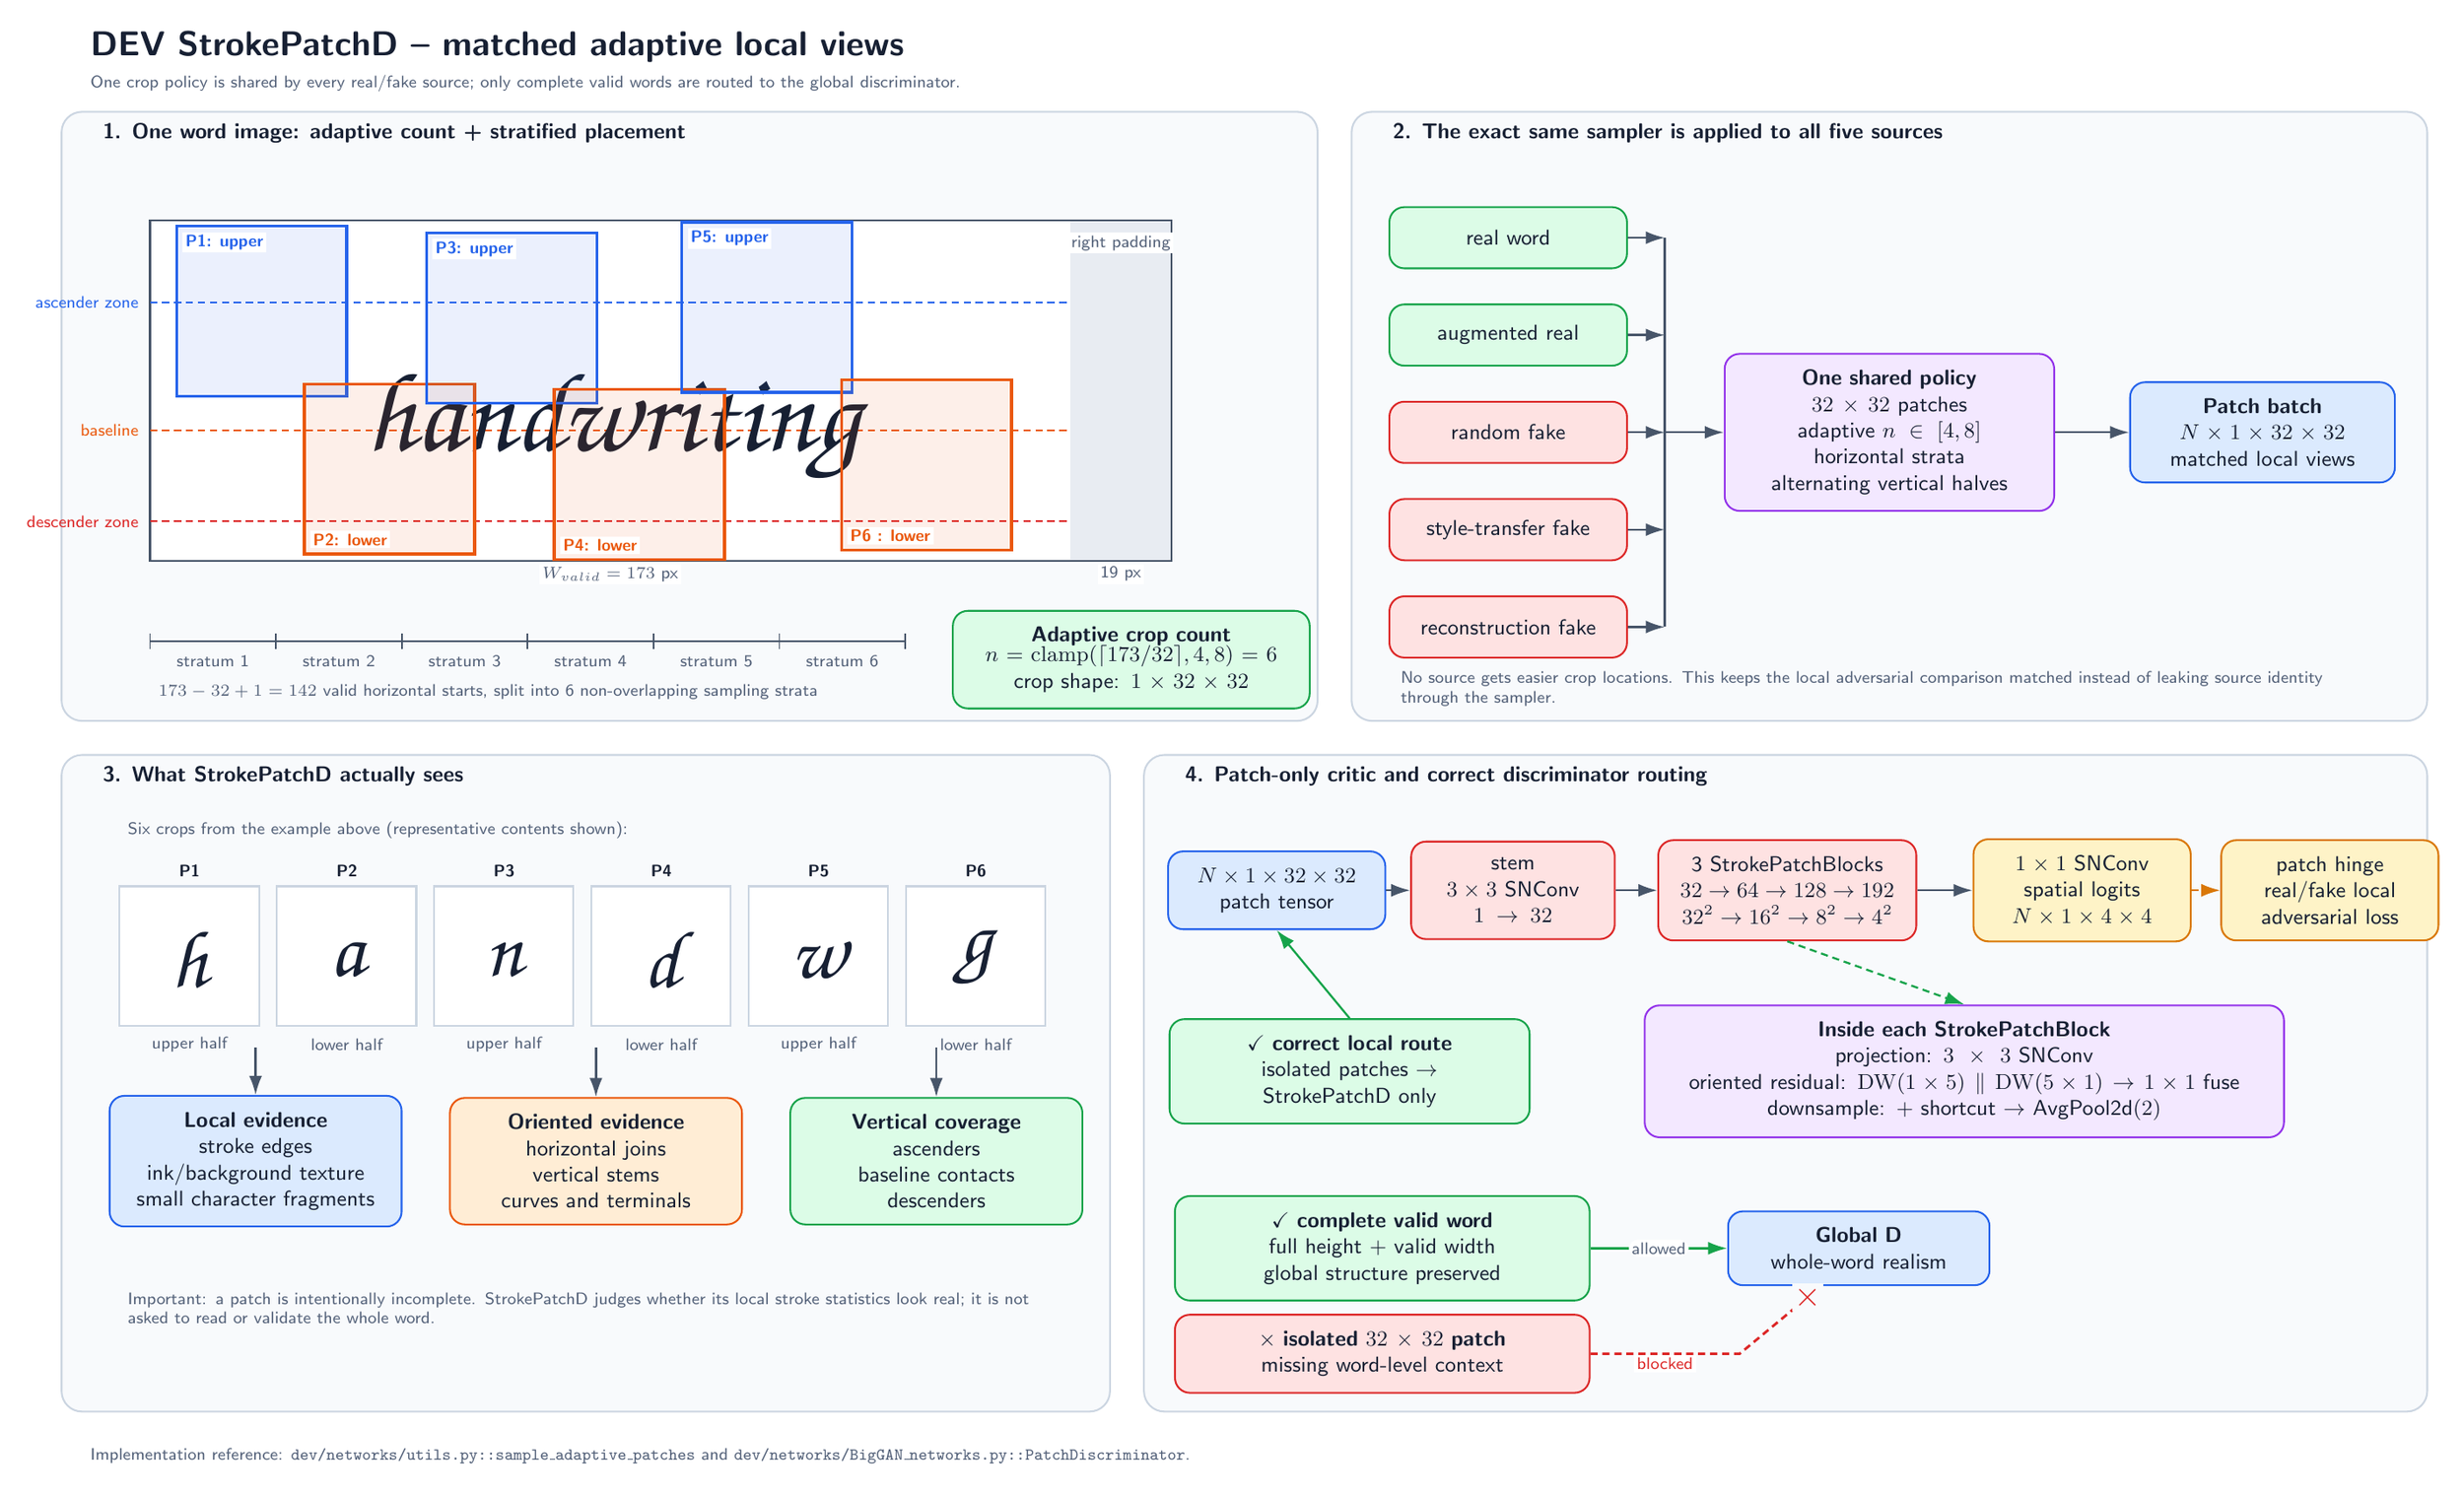
\begin{tikzpicture}[x=1cm,y=1cm]
  \node[font=\sffamily\bfseries\Large, text=DevInk, anchor=west]
    at (0,20.15) {DEV StrokePatchD -- matched adaptive local views};
  \node[devnote, anchor=west]
    at (0,19.62) {One crop policy is shared by every real/fake source; only complete valid words are routed to the global discriminator.};

  % Four fixed panels keep the information hierarchy and all connector lanes clear.
  \draw[devgroup] (-0.30,10.25) rectangle (18.15,19.20);
  \draw[devgroup] (18.65,10.25) rectangle (34.45,19.20);
  \draw[devgroup] (-0.30,0.10) rectangle (15.10,9.75);
  \draw[devgroup] (15.60,0.10) rectangle (34.45,9.75);

  \node[devgrouptitle, anchor=west] at (0.10,18.88)
    {1. One word image: adaptive count + stratified placement};
  \node[devgrouptitle, anchor=west] at (19.05,18.88)
    {2. The exact same sampler is applied to all five sources};
  \node[devgrouptitle, anchor=west] at (0.10,9.43)
    {3. What StrokePatchD actually sees};
  \node[devgrouptitle, anchor=west] at (16.00,9.43)
    {4. Patch-only critic and correct discriminator routing};

  % --------------------------------------------------------------------------
  % Panel 1: concrete 64 x 192 example with W_valid=173 and six crops.
  % --------------------------------------------------------------------------
  \coordinate (imgSW) at (1.00,12.60);
  \coordinate (imgNE) at (16.00,17.60);
  \fill[white] (imgSW) rectangle (imgNE);
  \fill[DevPanelBorder!45] (14.5156,12.60) rectangle (16.00,17.60);
  \draw[draw=DevLine,line width=0.8pt] (imgSW) rectangle (imgNE);
  \draw[draw=DevContentBorder,densely dashed,line width=0.7pt]
    (1.00,16.40) -- (14.5156,16.40);
  \draw[draw=DevAllographBorder,densely dashed,line width=0.7pt]
    (1.00,14.52) -- (14.5156,14.52);
  \draw[draw=DevCriticBorder,densely dashed,line width=0.7pt]
    (1.00,13.18) -- (14.5156,13.18);

  \node[font=\fontfamily{pzc}\selectfont\fontsize{47}{49}\selectfont,
        text=DevInk, anchor=center]
    at (7.80,14.55) {handwriting};

  \node[devlabel, anchor=east, fill=none, text=DevContentBorder]
    at (0.88,16.40) {ascender zone};
  \node[devlabel, anchor=east, fill=none, text=DevAllographBorder]
    at (0.88,14.52) {baseline};
  \node[devlabel, anchor=east, fill=none, text=DevCriticBorder]
    at (0.88,13.18) {descender zone};
  \node[devlabel, anchor=north] at (15.26,17.43) {right padding};
  \node[devlabel, anchor=north] at (7.76,12.56)
    {$W_{valid}=173$ px};
  \node[devlabel, anchor=north] at (15.26,12.56)
    {19 px};

  % Crop windows. Patch scale: 32 px = 2.5 cm. Odd crops sample the upper
  % vertical-position half; even crops sample the lower half.
  \foreach \x/\y/\id in {
    1.3906/15.02/1,
    3.2656/12.70/2,
    5.0625/14.92/3,
    6.9375/12.62/4,
    8.8125/15.08/5,
    11.1563/12.76/6
  }{
    \ifodd\id
      \draw[draw=DevContentBorder,fill=DevContentBorder,fill opacity=0.09,
            line width=1.25pt] (\x,\y) rectangle ++(2.5,2.5);
      \node[font=\sffamily\bfseries\scriptsize,text=DevContentBorder,
            fill=white,inner sep=1.2pt,anchor=north west]
        at ($(\x,\y)+(0.08,2.42)$) {P\id: upper};
    \else
      \draw[draw=DevAllographBorder,fill=DevAllographBorder,fill opacity=0.09,
            line width=1.25pt] (\x,\y) rectangle ++(2.5,2.5);
      \node[font=\sffamily\bfseries\scriptsize,text=DevAllographBorder,
            fill=white,inner sep=1.2pt,anchor=south west]
        at ($(\x,\y)+(0.08,0.08)$) {P\id: lower};
    \fi
  }

  % Horizontal start-position strata: 173 - 32 + 1 = 142 valid starts.
  \draw[draw=DevLine,line width=0.7pt] (1.00,11.42) -- (12.0938,11.42);
  \foreach \k in {0,...,6}{
    \draw[draw=DevLine,line width=0.65pt]
      ($(1.00,11.42)+(\k*1.84897,-0.12)$) -- ++(0,0.24);
  }
  \foreach \k in {1,...,6}{
    \node[devlabel, fill=none]
      at ($(1.00,11.42)+(\k*1.84897-0.9245,-0.30)$) {stratum \k};
  }
  \node[devnote, anchor=west] at (1.00,10.68)
    {$173-32+1=142$ valid horizontal starts, split into 6 non-overlapping sampling strata};

  \node[devstable, text width=4.6cm, anchor=west] at (12.78,11.15)
    {\textbf{Adaptive crop count}\\[-1mm]
     $n=\mathrm{clamp}(\lceil173/32\rceil,4,8)=6$\\
     crop shape: $1\times32\times32$};

  % --------------------------------------------------------------------------
  % Panel 2: five matched sources fan into one sampler.
  % --------------------------------------------------------------------------
  \node[devstable, text width=2.85cm] (real) at (20.95,17.35)
    {real word};
  \node[devstable, text width=2.85cm] (aug) at (20.95,15.92)
    {augmented real};
  \node[devcritic, text width=2.85cm] (rand) at (20.95,14.49)
    {random fake};
  \node[devcritic, text width=2.85cm] (transfer) at (20.95,13.06)
    {style-transfer fake};
  \node[devcritic, text width=2.85cm] (recn) at (20.95,11.63)
    {reconstruction fake};

  \coordinate (sourcebus) at (23.25,14.49);
  \draw[draw=DevLine,line width=0.85pt] (23.25,11.63) -- (23.25,17.35);
  \foreach \s in {real,aug,rand,transfer,recn}{
    \draw[devflow] (\s.east) -- (sourcebus |- \s.east);
  }

  \node[devstyle, text width=4.2cm] (sharedsampler) at (26.55,14.49)
    {\textbf{One shared policy}\\$32\times32$ patches\\adaptive $n\in[4,8]$\\horizontal strata\\alternating vertical halves};
  \draw[devflow] (sourcebus) -- (sharedsampler);

  \node[devcontent, text width=3.25cm] (patchbatch) at (32.03,14.49)
    {\textbf{Patch batch}\\$N\times1\times32\times32$\\matched local views};
  \draw[devflow] (sharedsampler) -- (patchbatch);
  \node[devnote, text width=13.8cm, anchor=west] at (19.25,10.72)
    {No source gets easier crop locations. This keeps the local adversarial comparison matched instead of leaking source identity through the sampler.};

  % --------------------------------------------------------------------------
  % Panel 3: representative local views, with explicit semantics.
  % --------------------------------------------------------------------------
  \node[devnote, anchor=west] at (0.55,8.64)
    {Six crops from the example above (representative contents shown):};

  \foreach \x/\label/\band/\glyph in {
    0.55/P1/upper/h,
    2.86/P2/lower/a,
    5.17/P3/upper/n,
    7.48/P4/lower/d,
    9.79/P5/upper/w,
    12.10/P6/lower/g
  }{
    \fill[white] (\x,5.77) rectangle ++(2.05,2.05);
    \draw[draw=DevPanelBorder,line width=0.75pt] (\x,5.77) rectangle ++(2.05,2.05);
    \node[font=\fontfamily{pzc}\selectfont\fontsize{34}{34}\selectfont,
          text=DevInk] at ($(\x,5.77)+(1.03,0.98)$) {\glyph};
    \node[font=\sffamily\bfseries\scriptsize,text=DevInk]
      at ($(\x,5.77)+(1.03,2.28)$) {\label};
    \node[devlabel, fill=none]
      at ($(\x,5.77)+(1.03,-0.28)$) {\band\ half};
  }

  \node[devcontent, text width=3.65cm] (localone) at (2.55,3.78)
    {\textbf{Local evidence}\\stroke edges\\ink/background texture\\small character fragments};
  \node[devallograph, text width=3.65cm] (localtwo) at (7.55,3.78)
    {\textbf{Oriented evidence}\\horizontal joins\\vertical stems\\curves and terminals};
  \node[devstable, text width=3.65cm] (localthree) at (12.55,3.78)
    {\textbf{Vertical coverage}\\ascenders\\baseline contacts\\descenders};
  \draw[devflow] (2.55,5.45) -- (localone.north);
  \draw[devflow] (7.55,5.45) -- (localtwo.north);
  \draw[devflow] (12.55,5.45) -- (localthree.north);

  \node[devnote, text width=13.7cm, anchor=west] at (0.55,1.62)
    {Important: a patch is intentionally incomplete. StrokePatchD judges whether its local stroke statistics look real; it is not asked to read or validate the whole word.};

  % --------------------------------------------------------------------------
  % Panel 4: lightweight anisotropic critic and explicit routing rule.
  % --------------------------------------------------------------------------
  \node[devcontent, text width=2.55cm] (ptensor) at (17.55,7.76)
    {$N\times1\times32\times32$\\patch tensor};
  \node[devcritic, text width=2.35cm] (stem) at (21.02,7.76)
    {stem\\$3\times3$ SNConv\\$1\rightarrow32$};
  \node[devcritic, text width=3.15cm] (blocks) at (25.05,7.76)
    {3 StrokePatchBlocks\\$32\rightarrow64\rightarrow128\rightarrow192$\\$32^2\rightarrow16^2\rightarrow8^2\rightarrow4^2$};
  \node[devloss, text width=2.55cm] (logits) at (29.38,7.76)
    {$1\times1$ SNConv\\spatial logits\\$N\times1\times4\times4$};
  \node[devloss, text width=2.55cm] (hinge) at (33.02,7.76)
    {patch hinge\\real/fake local\\adversarial loss};
  \draw[devflow] (ptensor) -- (stem);
  \draw[devflow] (stem) -- (blocks);
  \draw[devflow] (blocks) -- (logits);
  \draw[devlossflow] (logits) -- (hinge);

  \node[devstable, text width=4.65cm] (correctpatch) at (18.62,5.10)
    {\textbf{$\checkmark$ correct local route}\\isolated patches $\rightarrow$ StrokePatchD only};
  \draw[devflow, draw=DevStableBorder] (correctpatch.north) -- (ptensor.south);

  \node[devstyle, text width=8.75cm] (blockdetail) at (27.65,5.10)
    {\textbf{Inside each StrokePatchBlock}\\
     projection: $3\times3$ SNConv\\
     oriented residual: $\mathrm{DW}(1\times5)\;\Vert\;\mathrm{DW}(5\times1)
     \rightarrow1\times1$ fuse\\
     downsample: $+$ shortcut $\rightarrow$ AvgPool2d$(2)$};
  \draw[devaux] (blocks.south) -- (blockdetail.north);

  \node[devstable, text width=5.45cm] (fullword) at (19.10,2.50)
    {\textbf{$\checkmark$ complete valid word}\\full height + valid width\\global structure preserved};
  \node[devcontent, text width=3.20cm] (globald) at (26.10,2.50)
    {\textbf{Global D}\\whole-word realism};
  \draw[devflow, draw=DevStableBorder] (fullword) -- node[devlabel] {allowed} (globald);

  \node[devcritic, text width=5.45cm] (wrongpatch) at (19.10,0.95)
    {\textbf{$\times$ isolated $32\times32$ patch}\\missing word-level context};
  \draw[draw=DevCriticBorder,line width=1.05pt,densely dashed]
    (wrongpatch.east) -- node[devlabel,text=DevCriticBorder,below] {blocked}
    (24.35,0.95) -- (25.35,1.78);
  \node[font=\sffamily\bfseries\Large,text=DevCriticBorder,fill=DevPanel,
        inner sep=1pt] at (25.35,1.78) {$\times$};

  \node[devnote, anchor=west] at (0,-0.55)
    {Implementation reference: \texttt{dev/networks/utils.py::sample\_adaptive\_patches} and \texttt{dev/networks/BigGAN\_networks.py::PatchDiscriminator}.};
\end{tikzpicture}
\end{document}
